\addcontentsline{toc}{section}{Appendix} 

\chead{\textit{\nouppercase{Appendix}}}

\thispagestyle{plain} % surpress header on first page

\subsection{Appendix A: Tables}
\thispagestyle{plain} % surpress header on first page

\phantom{This text will be invisible} 
\hspace{20cm}
\begin{table}[H]
	\centering
	\caption{Overview of UQ literature}
	\label{tab:lit}
	\renewcommand{\arraystretch}{1.2}%
	\begin{tabular}{lc}
		\toprule
		Content                      & Number of articles \\ \midrule
		$Topics$                       &                    \\
		\qquad Climate economics            & 8                  \\
		\qquad Macroeconomics               & 4                 \\ \midrule
		$Analyses$                     &                    \\
		\qquad Uncertainty analysis      & 8                  \\
		\qquad Globabl sensitivity analysis & 7                  \\
		\qquad Local sensitivity analysis   & 2                  \\ \midrule
		$Measures$                     &                    \\
		\qquad Sobol' indices               & 6                  \\
		\qquad Univariate effects           & 4                  \\
		\qquad Density-based measures & 2                  \\ \midrule
		$Methods$                      &                    \\
		\qquad Monte Carlo sampling         & 7                  \\
		\qquad Latin hypercube sampling         & 3                  \\
		\qquad Surrogate model              & 7                  \\
		\qquad Polynomial chaos expansions  & 2                  \\
		\qquad Intrusive methods            & 2                  \\ \midrule
		& 14                 \\ \bottomrule
	\end{tabular}
\end{table}
\noindent

% increase spacing between table columns
\setlength{\tabcolsep}{18pt} %from 6
\begin{table}[H] 
	\centering
	\begin{threeparttable}
		\caption[Model Parameters]{Estimates for the distribution of input parameters}
		\label{tab:params}
		\renewcommand{\arraystretch}{1.2}%
		\begin{tabular}{cS[table-format=3.2]S[table-format=3.2]S[table-format=3.2]}
			\toprule
			{Parameter}     & {Mean}   & {Standard error (SE)} & {SE in KW94} \\ \midrule
			\textit{General} \\
			$\delta$ & 0.95   & 0.00084 & \textit{-}    \\    \midrule
			\textit{Blue-collar}\\    
			$\beta^b$ & 9.21   & .013            & 0.014      \\
			$\beta_e^b$ & 0.038  &    0.0011        & 0.0015       \\
			$\beta^b_b$ & 0.033  & 0.00044            & 0.00079       \\
			$\beta^b_{bb}$ & -0.0005 & 0.000013           & 0.000019       \\
			$\beta^b_w$ & 0.0    & 0.00067             & 0.0024      \\
			$\beta^b_{ww}$ & 0.0    & 0.000029           & 0.000096       \\ \midrule
			\textit{White-collar}\\
			$\beta^w$ & 8.48   & 0.0076             & 0.0123      \\
			$\beta^w_e$ & 0.07   & 0.00047          & 0.00096       \\
			$\beta^w_w$ & 0.067  & 0.00055            & 0.00090      \\
			$\beta^w_{ww}$ & -0.001  & 0.000017           & 0.000070     \\
			$\beta^w_b$ & 0.022  & 0.00033           & 0.0010      \\
			$\beta^w_{bb}$ & -0.0005 & 0.000021         & 0.000030      \\ \midrule
			\textit{Education} \\
			$\beta^e$     & 0.0    & 330                & 459       \\
			$\beta_{he}^e$     & 0.0    & 155               & 410       \\
			$\beta_{re}^e$     & -4000   & 202                & 660       \\ \midrule
			\textit{Home} \\
			$\beta^h$    & 17750  & 390                & 1442      \\ \midrule
			\multicolumn{4}{l}{\textit{Lower Triangular Cholesky Matrix}} \\
			$c_{1}$      & 0.2    & 0.0015             & 0.0056      \\
			$c_{2}$      & 0.25    & 0.0013             & 0.0046     \\
			$c_{3}$      & 1500   & 108             & 350      \\
			$c_{4}$      & 1500    & 176              & 786      \\
			$c_{1,2}$     & 0.0    & 0.0064              & 0.023     \\
			$c_{1,3}$      & 0.0   & 145               & 0.412      \\
			$c_{2,3}$      & 0.0    & 116             &  0.379     \\
			$c_{1,4}$      & 0.0    & 235             &   0.911    \\
			$c_{2,4}$      & 0.0    & 131            & 0.624      \\
			$c_{3,4}$      & 0.0   & 178                & 0.870       \\ \bottomrule
		\end{tabular}
	\end{threeparttable}
\end{table}

% Please add the following required packages to your document preamble:
% \usepackage{booktabs}
\setlength{\tabcolsep}{12pt} %from 6
\begin{table}[H]
	\centering
	\caption{Replication and Validation - trajectory design}
	\label{tab:repval1}
	\renewcommand{\arraystretch}{1.2}%
	\begin{threeparttable}
		\begin{tabular}{cS[table-format=3.2]S[table-format=3.2]S[table-format=3.2]S[table-format=3.2]}
			\toprule
			{Measure}     & {GM'17}   & {Repl. $\mu^{*}$}\tnote{$\dagger$} & {Repl. $\sigma$}\tnote{$\ddagger$} & {S'20} \\ \midrule
			
			
			& 1.20  & 1.36         & 0.83         & 1.00 \\
			\qquad $\mu^{*,ind}$                               & 1.30  & 1.48         & 0.91         & 1.00 \\
			& 3.20  & 3.11         & 1.94         & 1.00 \\
			&&&& \\
			& 0.55  & 0.00         & 0.56         & 0.00 \\
			\qquad $\sigma^{ind}$                            & 0.60  & 0.00         & 0.62         & 0.00 \\
			& 1.30  & 0.00         & 1.32         & 0.00 \\
			&&&& \\
			& 14.90 & 16.20        & 9.97         & 2.30 \\
			\qquad $\mu^{*,full}$                              & 12.50 & 13.45        & 8.31         & 1.91 \\
			& 10.00 & 9.93         & 6.18         & 1.41 \\
			&&&& \\
			& 6.50  & 0.00         & 6.74         & 0.00 \\
			\qquad $\sigma^{full}$                           & 5.50  & 0.00         & 5.63         & 0.00 \\
			& 4.00  & 0.00         & 4.20         & 0.00 \\		
			\bottomrule	
		\end{tabular}
		\begin{tablenotes}
			
			\item[$\dagger$] \footnotesize $0^{num}=0.00001$ and $l=4$. 
			\item[$\ddagger$] $0^{num}=0.00000001$ and $l=24$.\par
			
		\end{tablenotes}
	\end{threeparttable}
\end{table}

\phantom{This text will be invisible} 
\hspace{5cm} %linebreak.
% Please add the following required packages to your document preamble:
% \usepackage{booktabs}
\setlength{\tabcolsep}{12pt} %from 6
\begin{table}[H]
	\centering
	\caption{Replication and Validation - radial design}
	\label{tab:repval2}
	\renewcommand{\arraystretch}{1.2}%
	\begin{tabular}{cS[table-format=3.2]S[table-format=3.2]S[table-format=3.2]}
		\toprule
		{Measure}     & {GM'17}   & {Replication}  & {S'20} \\ 
		\midrule
		
		& 0.60  & 0.57         &  1.00 \\
		\qquad $\mu^{*,ind}$                               & 0.75  & 0.85         &  1.00 \\
		& 1.50  & 1.31         &  1.00 \\
		&&& \\
		& 0.20   & 0.10         &  0.00 \\
		\qquad $\sigma^{ind}$                            & 0.30   & 0.41         &  0.00 \\
		& 0.85  & 0.22         & 0.00 \\
		&&& \\
		& 7.50  & 6.84         &  2.30 \\
		\qquad $\mu^{*,full}$                              & 6.80   & 7.77         &  1.91 \\
		& 4.75  & 4.19         &  1.41 \\
		&&& \\
		& 2.90  & 1.15         &  0.00 \\
		\qquad $\sigma^{full}$                           & 2.65  & 3.68         &  0.00 \\
		& 2.50   & 0.70         &  0.00 \\ \bottomrule
	\end{tabular}
\end{table}

\newpage
\phantom{This text will be invisible} 
\vspace{10mm} %5mm vertical space
% Please add the following required packages to your document preamble:
% \usepackage{booktabs}
\begin{table}[H]
	\centering
	\caption{Comparison of sensitivity measures for a linear function}
	\label{tab:bad-mu}
	\begin{tabular}{@{}lccc@{}}
		\toprule
		Parameters & $S_i^T$ & $\gamma_i^*$ & $(\mu_i^* \frac{\sigma_{X_i}}{\sigma_Y})^2$ \\ \midrule
		$X_1$ & $9$                       & $3$   & $9$   \\
		$X_2$ & $8$                       & $2$   & $8$   \\
		$X_3$ & $9$                       & $1$   & $9$   \\ \bottomrule
	\end{tabular}
\end{table}

\newpage
\setlength{\tabcolsep}{22pt} %from 6
\begin{table}[H] 
	\centering
	\begin{threeparttable}
		\caption[Quantitative GSA measures by \cite{ge2017extending}]{EE-based measures by \cite{ge2017extending} for 100 trajectories}
		\label{tab:kw94gm17}
		\renewcommand{\arraystretch}{1.2}%
		\begin{tabular}{cS[table-format=3.2]S[table-format=3.2]@{\hskip 0.7in}|@{\hskip 0.5in}S[table-format=3.2]S[table-format=3.2]}
			
			{Parameter}     & {$\mu^{*,full}_T$}   & {$\mu^{*,ind}_T$} & {$\sigma^{*,full}_T$} & {$\sigma^{*,ind}_T$}\\ \midrule
			\textit{General} \\
			$\delta$ & 53.40   & 0.00 & 69.23 & 0.09   \\    \midrule
			\textit{Blue-collar}\\    
			$\beta^b$ & 3.55   & 0.05            & 4.38 & 0.07    \\
			$\beta_e^b$ & 39.84  &    0.05        & 49.69  & 0.07    \\
			$\beta^b_b$ & 77.21  & 0.05            & 90.23  & 0.07    \\
			$\beta^b_{bb}$ & 2616.50 & 0.05           & 3357.92  & 0.06     \\
			$\beta^b_w$ & 94.74    & 0.05             & 113.49  &  0.06  \\
			$\beta^b_{ww}$ & 1136.58    & 0.03          & 1405.94 &  0.04    \\ \midrule
			\textit{White-collar}\\
			$\beta^w$ & 5.07   & 0.05            & 6.42 &  0.06   \\
			$\beta^w_e$ & 90.25   & 0.07          & 111.50 &  0.08    \\
			$\beta^w_w$ & 82.88  & 0.05            & 103.66 &  0.07   \\
			$\beta^w_{ww}$ & 2444.13  & 0.06           & 3044.69 & 0.07   \\
			$\beta^w_b$ & 452.91 & 0.07           & 490.31 &  0.09   \\
			$\beta^w_{bb}$ & 4317.58 & 0.05         & 4851.54 &  0.06   \\ \midrule
			\textit{Education} \\
			$\beta^e$     & 0.00    & 0.09             & 0.00&  0.10   \\
			$\beta_{he}^e$     & 0.00    & 0.11              & 0.00  & 0.13    \\
			$\beta_{re}^e$     & 0.00  & 0.04               & 0.000  &   0.09  \\ \midrule
			\textit{Home} \\
			$\beta^h$    & 0.00  & 0.04                 & 0.00  & 0.05     \\ \midrule
			\multicolumn{4}{l}{\textit{Lower Triangular Cholesky Matrix}} \\
			$c_{1}$      & 27.94    & 0.07             & 33.72 &  0.08   \\
			$c_{2}$      & 31.89   & 0.05             & 38.58 & 0.06   \\
			$c_{3}$      & 0.00   & 0.06             & 0.00 & 0.07    \\
			$c_{4}$      & 0.00    & 0.04              & 0.00 & 0.09    \\
			$c_{1,2}$     & 12.41   & 0.06            & 14.33 &  0.08  \\
			$c_{1,3}$      & 0.00   & 0.09              & 0.00 &  0.10   \\
			$c_{2,3}$      & 0.00    & 0.05             &  0.00 &   0.06 \\
			$c_{1,4}$      & 0.00    & 0.04            &   0.00 &  0.05 \\
			$c_{2,4}$      & 0.00    & 0.03           & 0.00  &  0.03  \\
			$c_{3,4}$      & 0.00   & 0.04                & 0.00  &  0.05   \\ \bottomrule
		\end{tabular}
	\end{threeparttable}
\end{table}


\newpage
\setlength{\tabcolsep}{22pt} %from 6
\begin{table}[H] 
	\centering
	\begin{threeparttable}
		\captionsetup{format=hang}
		\caption[Quantitative GSA measures for the Occupational Choice Model]{Mean absolute correlated and uncorrelated elementary effects. The results are computed from 100 subsamples in trajectory and radial design.}
		\label{tab:devees}
		\renewcommand{\arraystretch}{1.2}%
		\begin{tabular}{cS[table-format=3.2]S[table-format=3.2]@{\hskip 0.7in}|@{\hskip 0.5in}S[table-format=3.2]S[table-format=3.2]}
			
			{Parameter}     & {$\mu^{*,c}_T$}   & {$\mu^{*,c}_R$} & {$\mu^{*,u}_T$} & {$\mu^{*,u}_R$}\\ \midrule
			\textit{General} \\
			$\delta$ & 17   & 23 & 476 & 415   \\    \midrule
			\textit{Blue-collar}\\    
			$\beta^b$ & 1   & 3            & 43 & 88    \\
			$\beta_e^b$ & 11  &    14        & 406  & 443    \\
			$\beta^b_b$ & 25  & 51            & 688  & 1169    \\
			$\beta^b_{bb}$ & 871 & 934           & 15540  & 17860     \\
			$\beta^b_w$ & 29    & 48             & 73  &  143  \\
			$\beta^b_{ww}$ & 389    & 460           & 869 &  1183    \\ \midrule
			\textit{White-collar}\\
			$\beta^w$ & 1   & 3            & 50 &  117   \\
			$\beta^w_e$ & 26   & 28          & 943 &  852    \\
			$\beta^w_w$ & 24  & 47            & 718 &  1521   \\
			$\beta^w_{ww}$ & 933  & 997           & 12257 & 18069   \\
			$\beta^w_b$ & 131 & 127           & 309 &  356   \\
			$\beta^w_{bb}$ & 1230 & 1352         & 2088 &  2477   \\ \midrule
			\textit{Education} \\
			$\beta^e$     & 0.0008    & 0.0002              & 0.001&  0.003   \\
			$\beta_{he}^e$     & 0.0001    & 0.0002              & 0.001  & 0.001    \\
			$\beta_{re}^e$     & 0.0003   & 0.0002               & 0.0003  &   0.0006  \\ \midrule
			\textit{Home} \\
			$\beta^h$    & 0.0003  & 0.0003                 & 0.00002  & 0.00002     \\ \midrule
			\multicolumn{4}{l}{\textit{Lower Triangular Cholesky Matrix}} \\
			$c_{1}$      & 8    & 16             & 18 &  37   \\
			$c_{2}$      & 8   & 11             & 22 & 24   \\
			$c_{3}$      & 0.0004   & 0.0004             & 0.0004 & 0.0007    \\
			$c_{4}$      & 0.0004    & 0.00008              & 0.0002 & 0.0003    \\
			$c_{1,2}$     & 4   & 4            & 10 &  10  \\
			$c_{1,3}$      & 0.0005   & 0.0006              & 0.0006 &  0.0005   \\
			$c_{2,3}$      & 0.0003    & 0.0005             &  0.0006 &   0.001 \\
			$c_{1,4}$      & 0.00004    & 0.00005            &   0.0004 &  0.0005 \\
			$c_{2,4}$      & 0.0001    & 0.0002           & 0.0001  &  0.0002  \\
			$c_{3,4}$      & 0.0001   & 0.0001                & 0.00008  &  0.0001   \\ \bottomrule
		\end{tabular}
	\end{threeparttable}
\end{table}


\subsection{Appendix B: Figures}
\thispagestyle{plain} % surpress header on first page

\vspace{10mm} %5mm vertical space
\begin{figure}[H]
	\caption{Timeline of events} \label{fig:order}
	\vspace{-0.0cm}
	
	\begin{center}        
		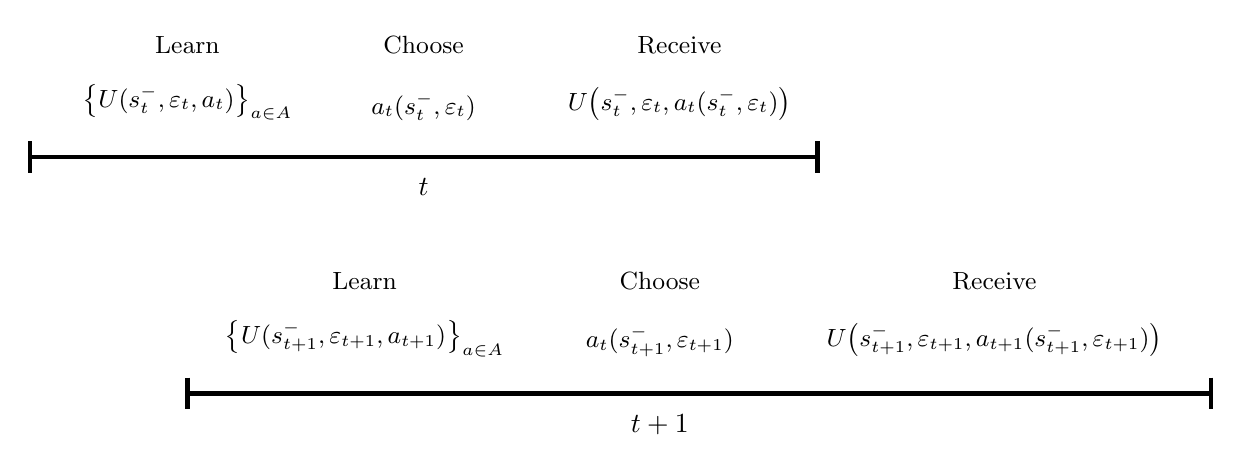
\begin{tikzpicture}
		% upper part
		\draw [ultra thick] (0,0) -- (10,0);
		\foreach \x in {0,10}
		\draw [ultra thick] (\x cm,0.2) -- (\x cm, -0.2);
		\small % derease fontsize
		\draw (2.0,0) node[above=0.35cm] {$\big\{U(\bold{s_t^-}, \pmb{\varepsilon_t},a_t)\big\}_{a \in A}$};
		\draw (5.0,0) node[above=0.35cm] {$a_t(\bold{s_t^-}, \pmb{\varepsilon_t})$};
		\draw (8.25,0) node[above=0.35cm] {$U\big(\bold{s_t^-}, \pmb{\varepsilon_t},a_t(\bold{s_t^-}, \pmb{\varepsilon_t})\big)$};
		
		\draw (2.0,0) node[above=1.2cm] {Learn};
		\draw (5.0,0) node[above=1.2cm] {Choose};
		\draw (8.25,0) node[above=1.2cm] {Receive};
		
		\normalsize %reincrease fontsize
		\draw (5.0,0) node[below=0.15cm] {$t$};
		
		%lower part
		\draw [ultra thick] (2.0,-3) -- (15,-3);
		\foreach \x in {2.0,15}
		\draw [ultra thick] (\x cm,-2.8) -- (\x cm, -3.2);
		\small % derease fontsize
		\draw (4.25,-3) node[above=0.35cm] {$\big\{U(\bold{s_{t+1}^-}, \pmb{\varepsilon_{t+1}},a_{t+1})\big\}_{a \in A}$};
		\draw (8.0,-3) node[above=0.35cm] {$a_t(\bold{s_{t+1}^-}, \pmb{\varepsilon_{t+1}})$};
		\draw (12.25,-3) node[above=0.35cm] {$U\big(\bold{s_{t+1}^-}, \pmb{\varepsilon_{t+1}},a_{t+1}(\bold{s_{t+1}^-}, \pmb{\varepsilon_{t+1}})\big)$};
		
		\draw (4.25,-3) node[above=1.2cm] {Learn};
		\draw (8.0,-3) node[above=1.2cm] {Choose};
		\draw (12.25,-3) node[above=1.2cm] {Receive};
		
		\normalsize %reincrease fontsize
		\draw (8.0,-3) node[below=0.15cm] {$t+1$};      
		
		%\draw (2.35,0) node[above=6pt, align=center] {(estimation \\ window]};
		\end{tikzpicture}
	\end{center}
\end{figure}

\vspace{20mm} %5mm vertical space


\begin{figure}[H]
	\caption{Correlations between estimates for important input parameters}
	\centering
	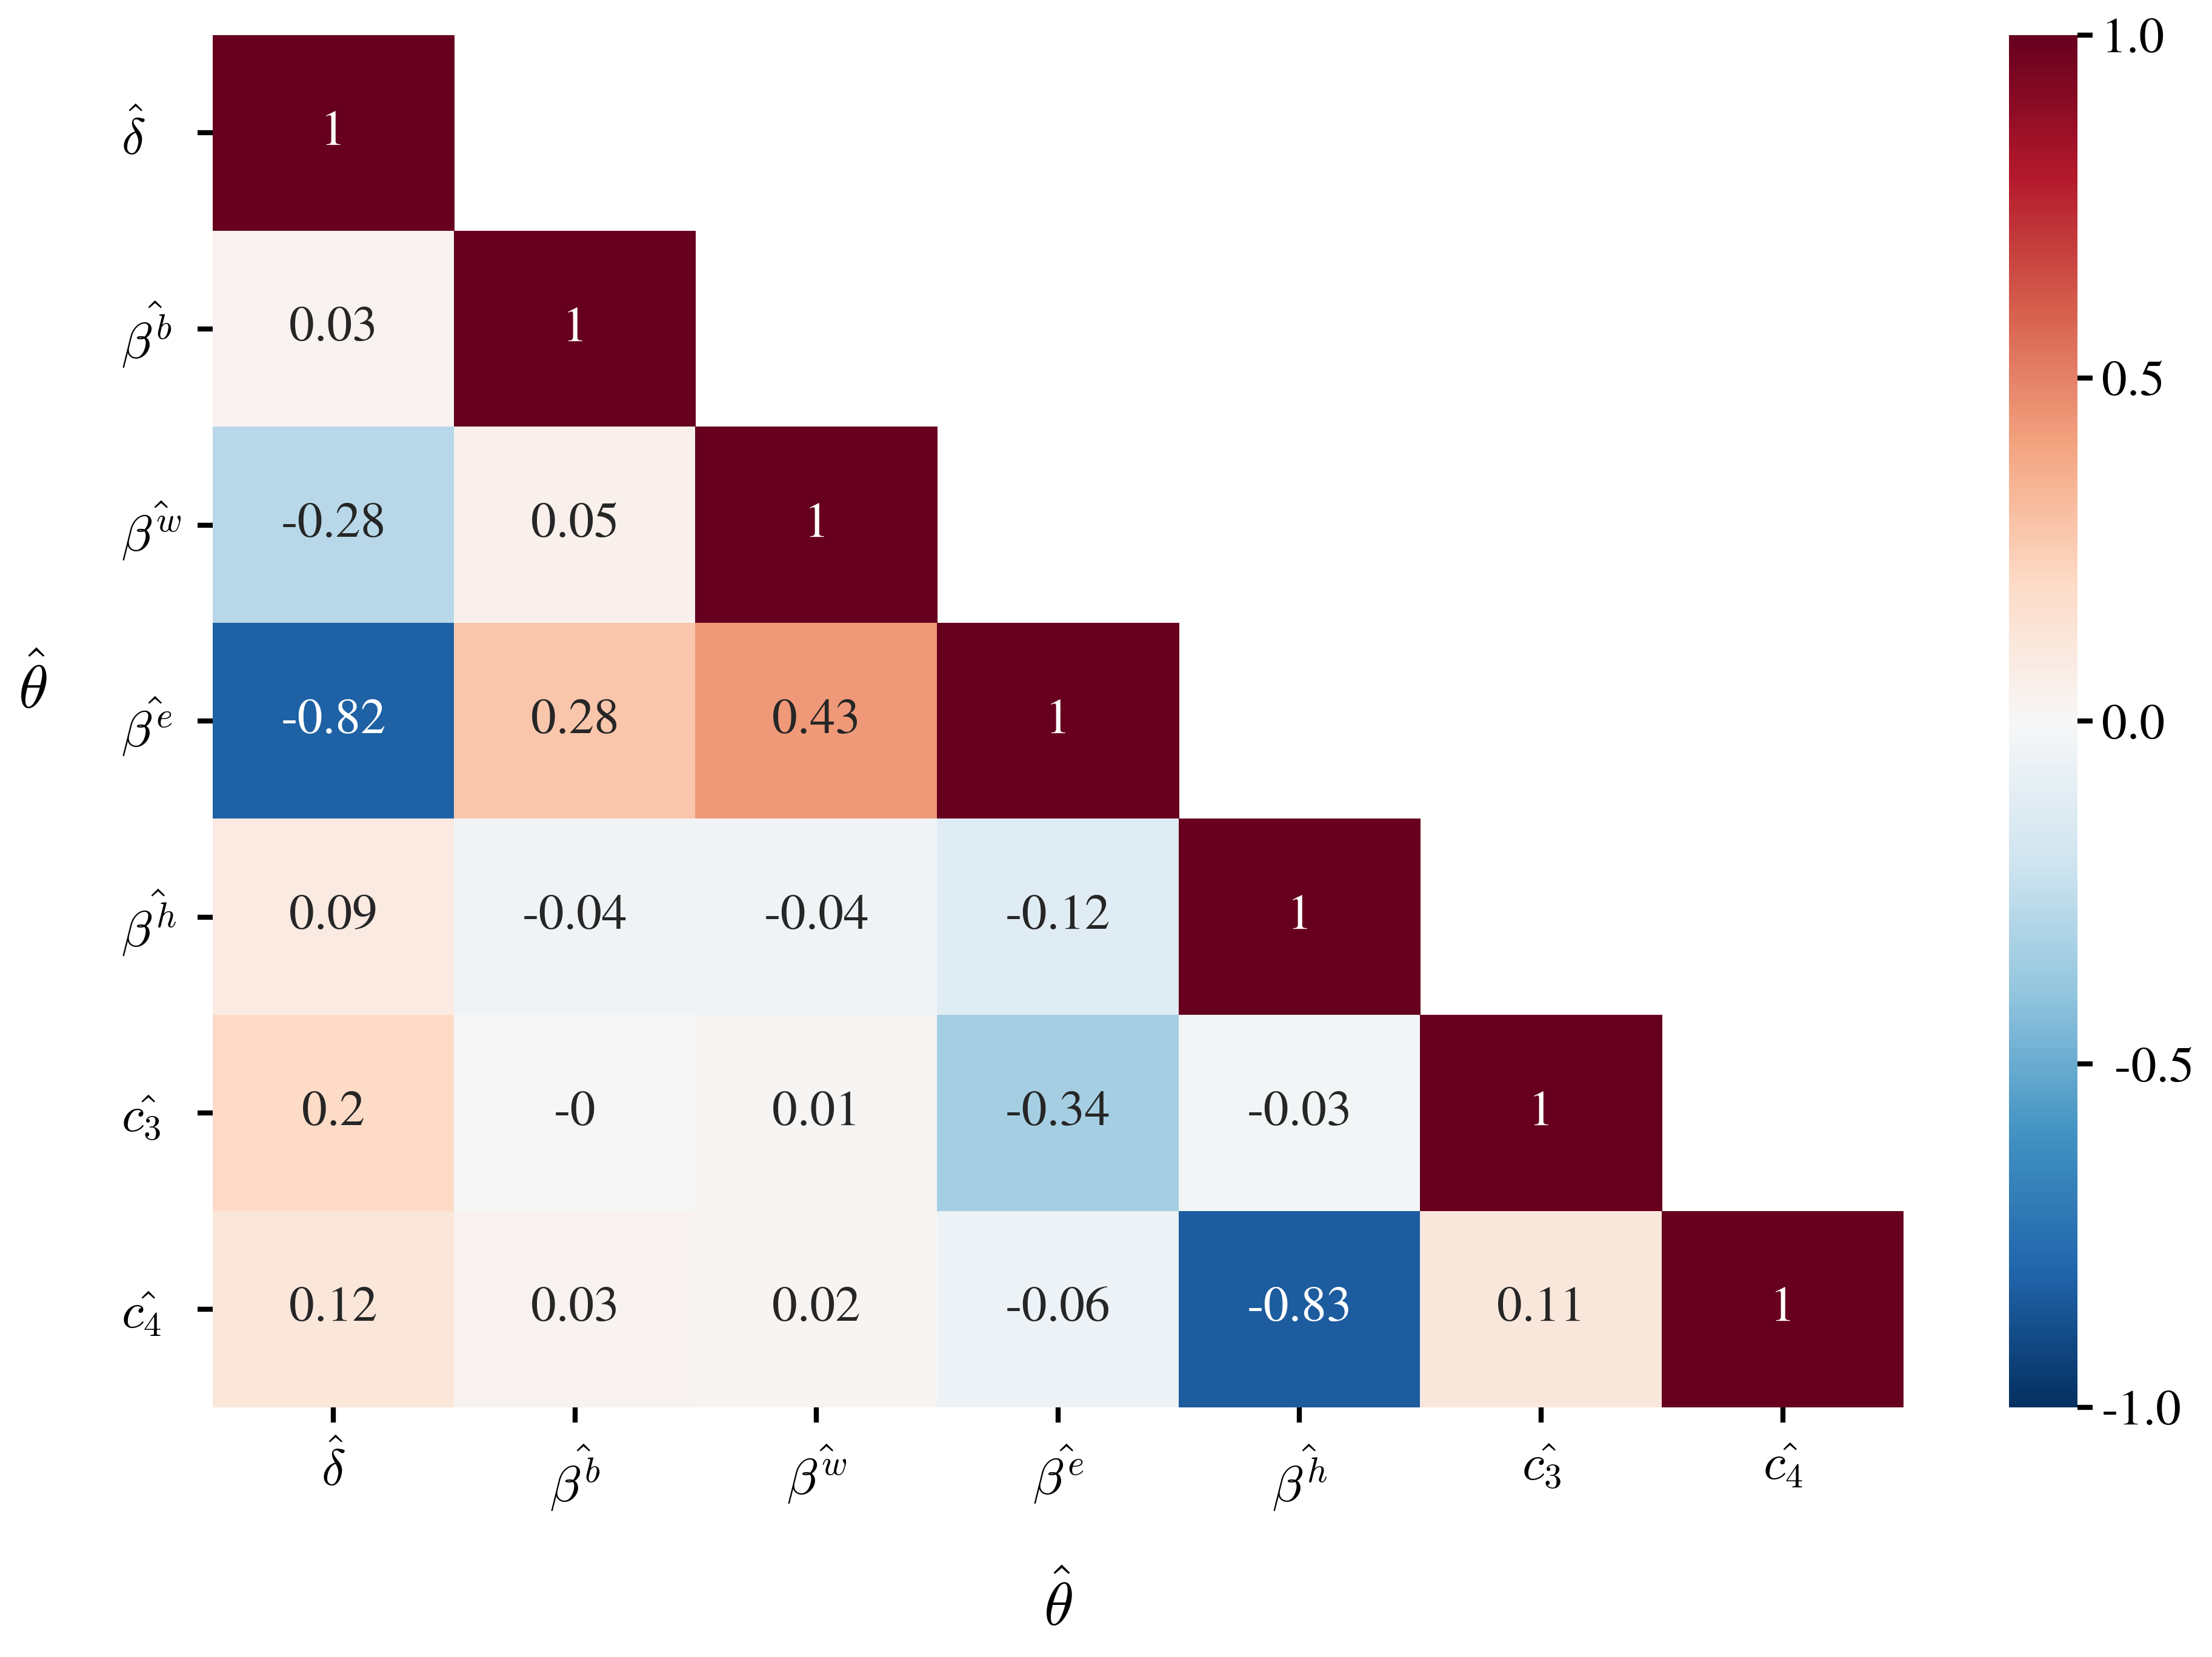
\includegraphics[scale=0.45]{../scrypy/figures/heatmap}
	\label{fig:corr}
\end{figure}
\newpage
\phantom{This text will be invisible} 
\vspace{20mm} %5mm vertical space
\begin{figure}[H]
	\caption[Comparison of shares of occupation decisions]{Comparison of shares of occupation decisions over time between scenarios}
	\centering
	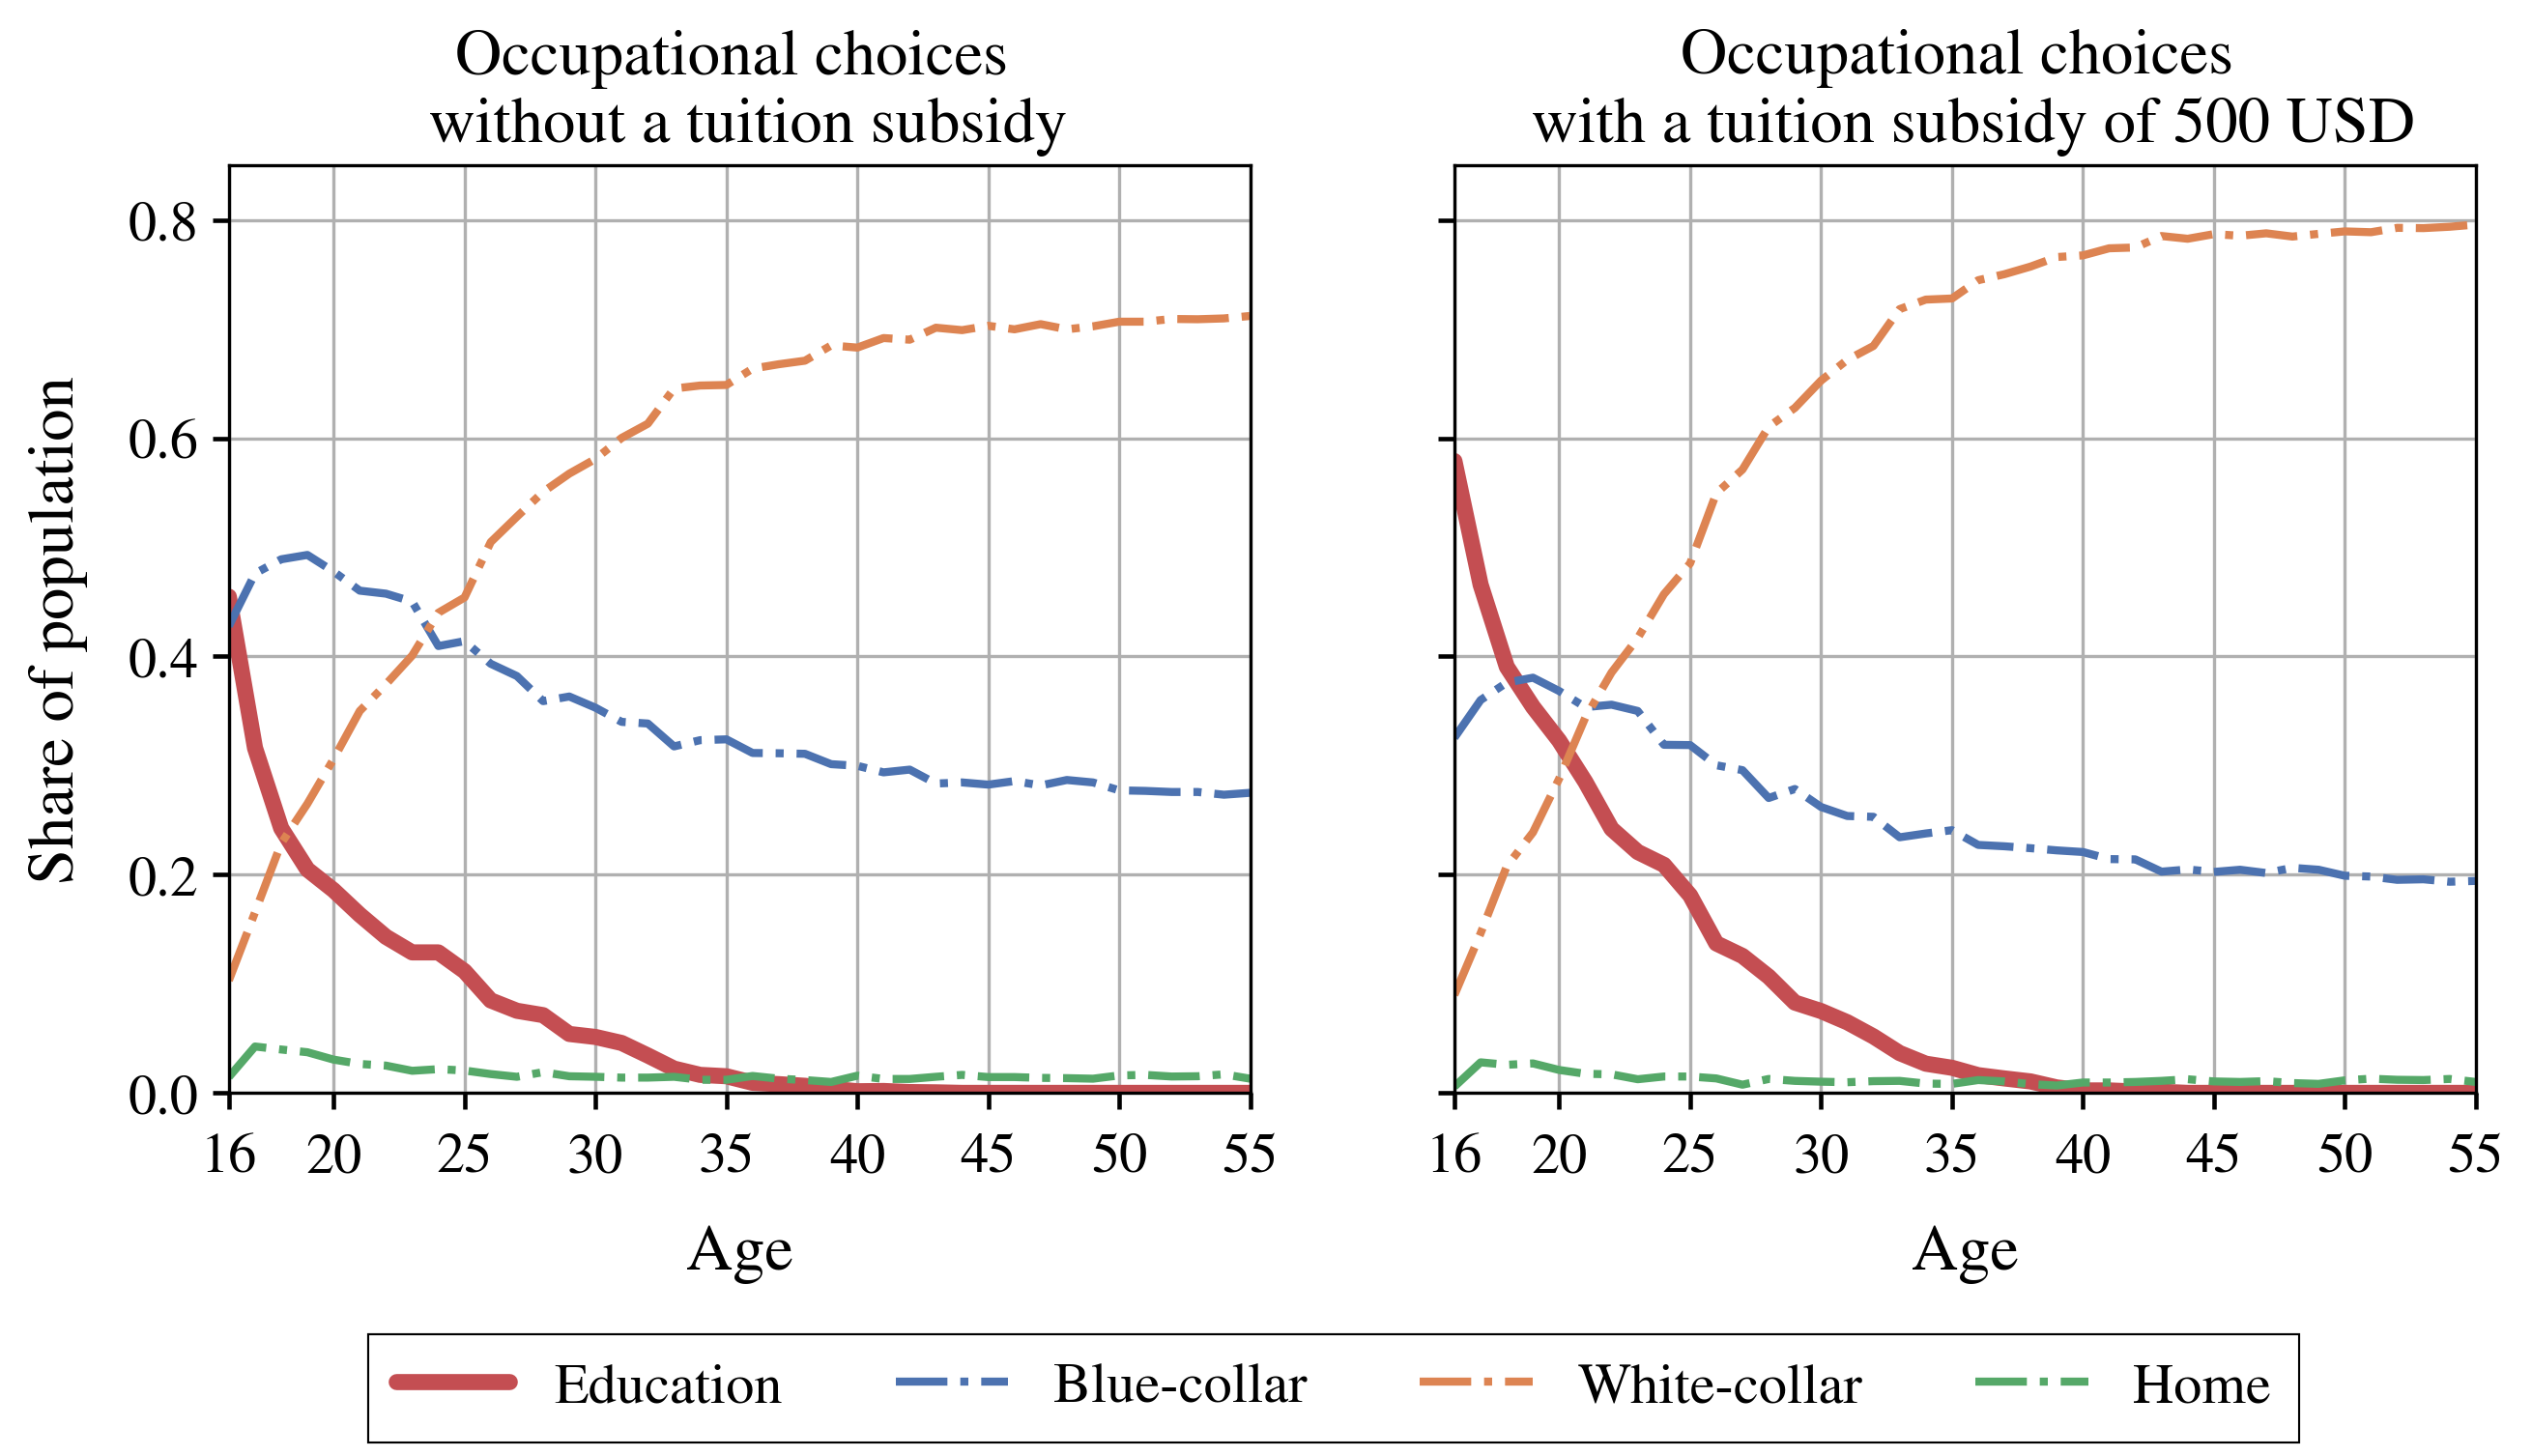
\includegraphics[scale=0.75]{../scrypy/figures/occ_choice_shares}
	\label{fig:paths}
\end{figure}

\vspace{10mm} %5mm vertical space

\begin{figure}[H]
	\caption[Grid points in standard normal sample]{Grid points in standard normal sample space for trajectory design with $l=4$}
	\centering
	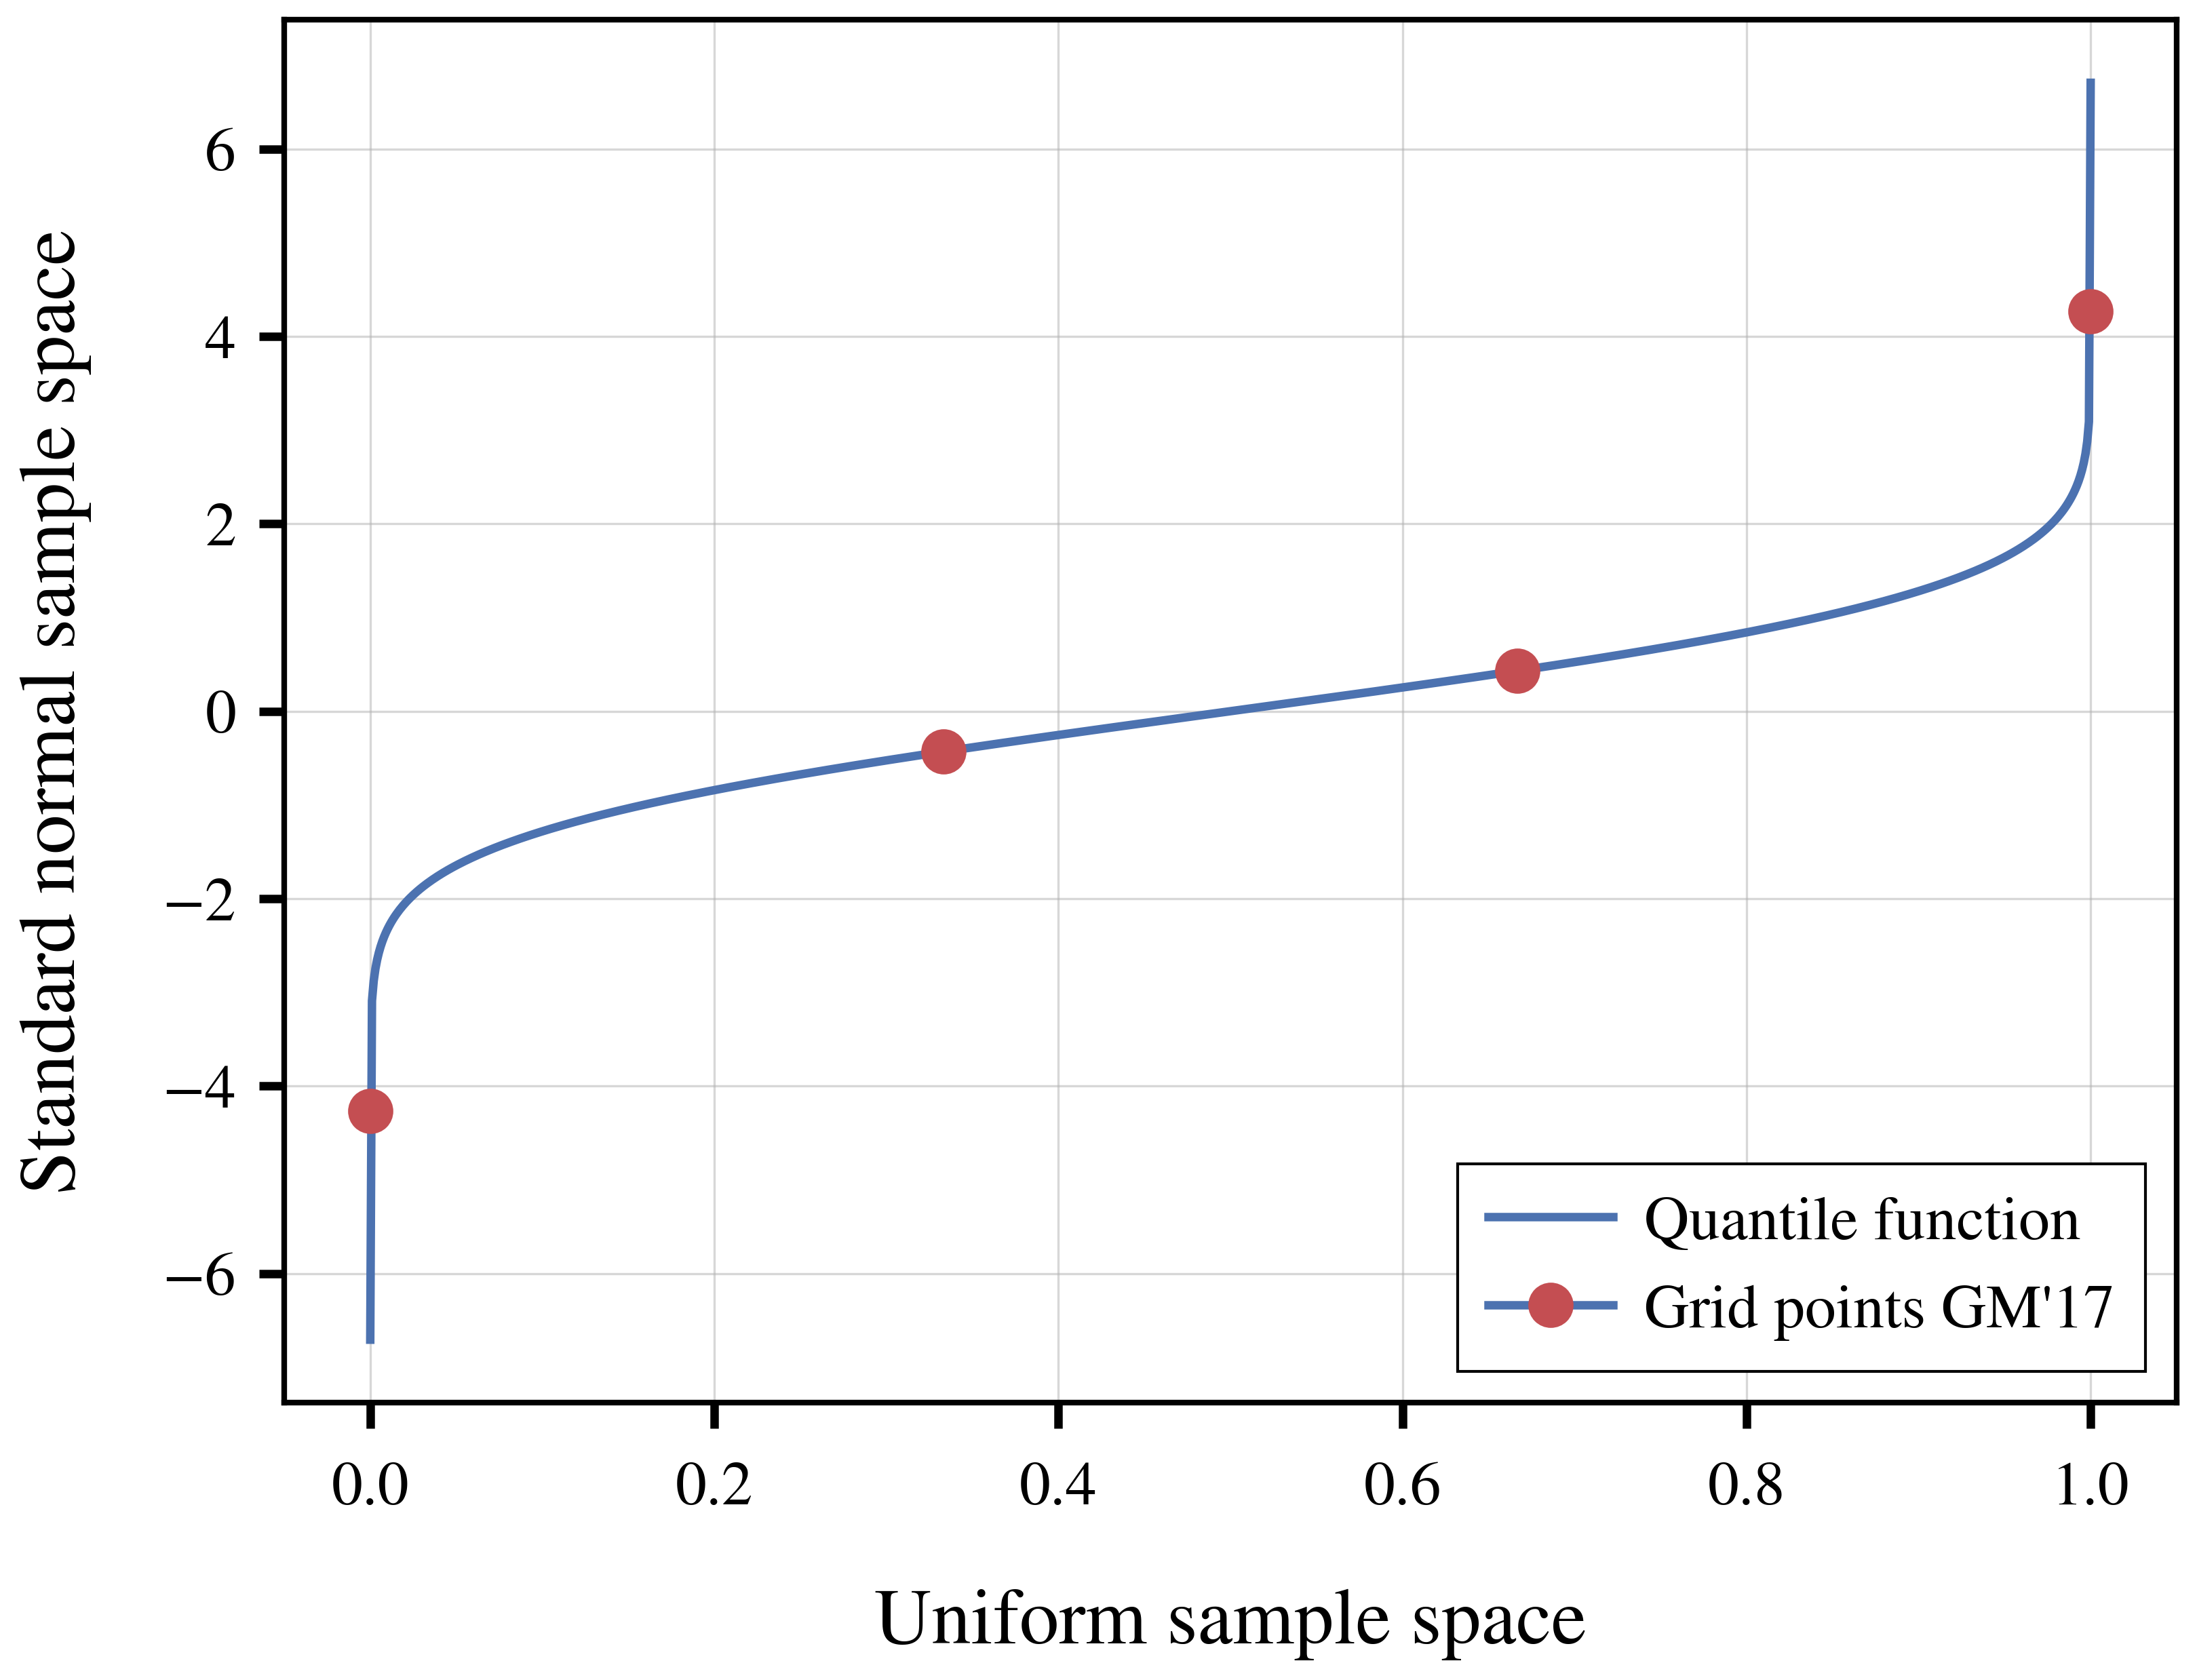
\includegraphics[scale=0.40]{../scrypy/figures/quantile_fct}
	\label{fig:invcdf}
\end{figure}



\begin{figure}[H]
	\captionsetup{format=hang}
	\caption[Comparison of uncertain shares of occupation decisions]{Comparison of shares of occupation decisions over time between scenarios including 99$\%$ confidence intervals}
	\centering
	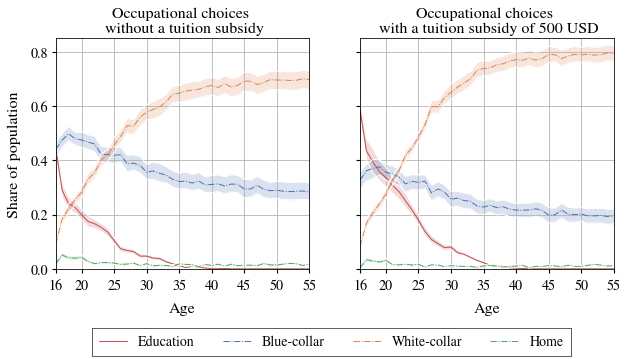
\includegraphics[scale=0.75]{../scrypy/figures/cone_plot_choice_shares}
	\label{fig:uq_paths}
\end{figure}

\vspace{10mm} %5mm vertical space

\begin{figure}[H]
	\caption{Probability distribution of QoI $Y$}
	\centering
	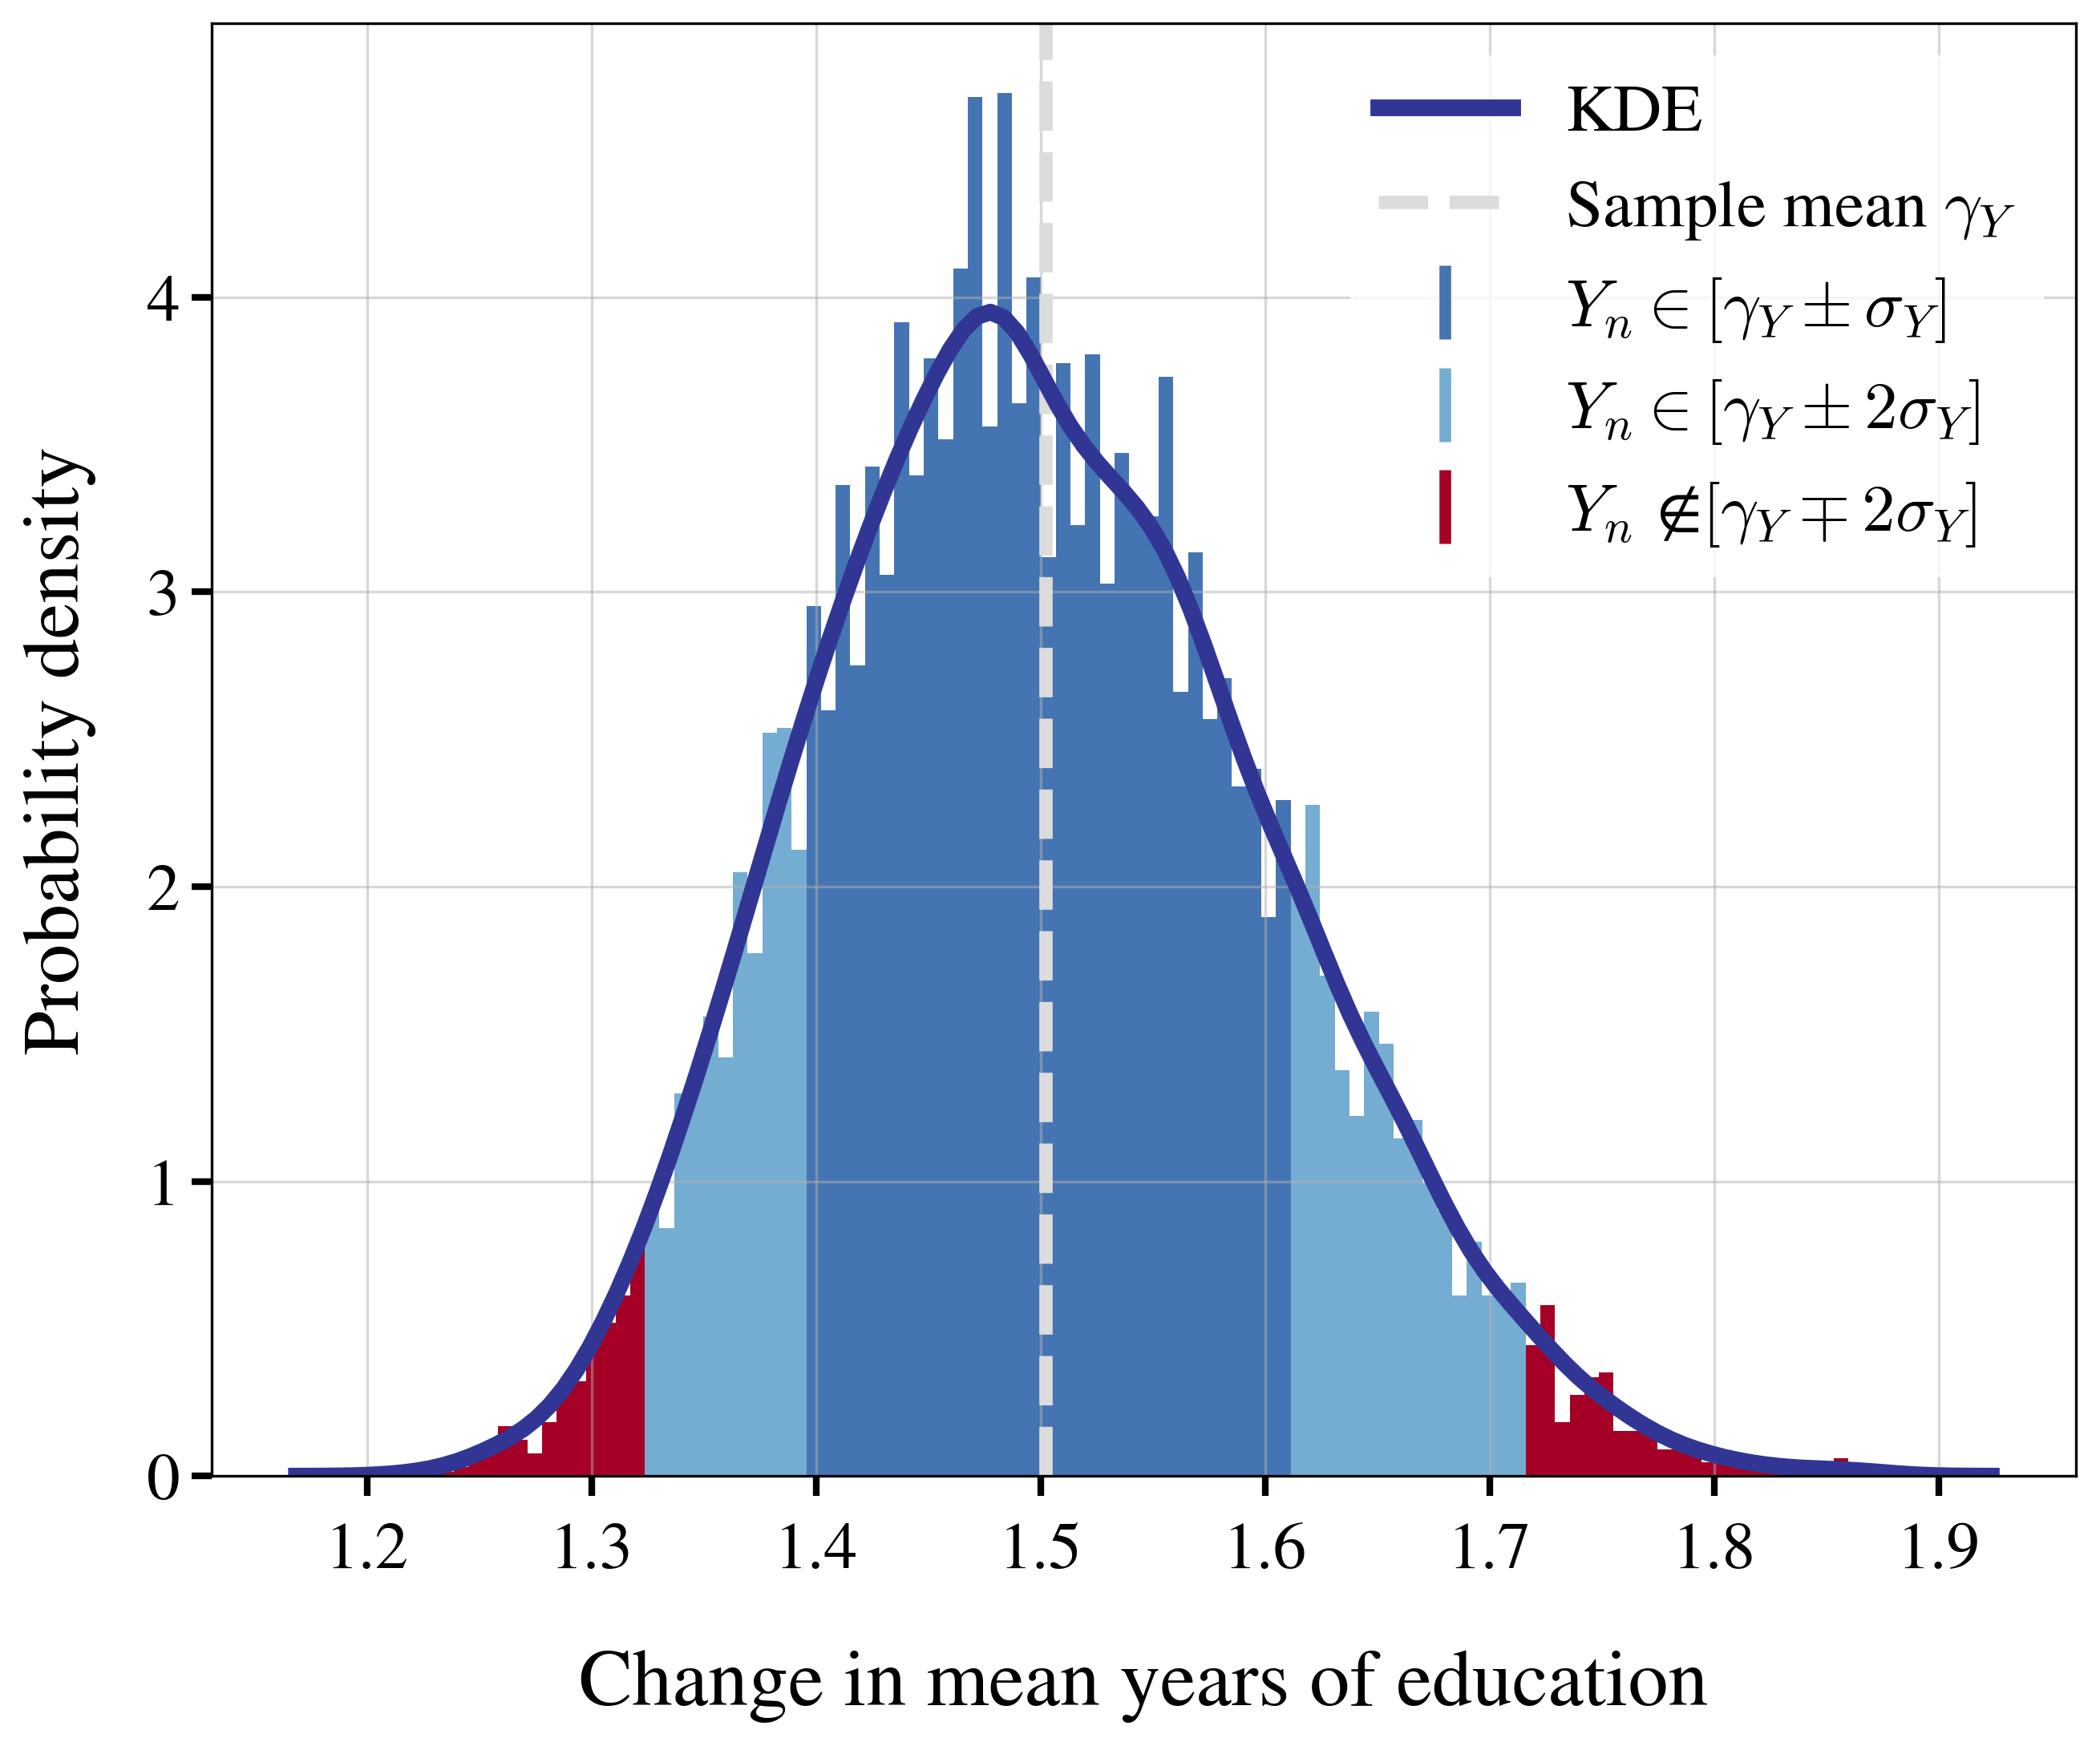
\includegraphics[scale=0.55]{../scrypy/figures/distplot}
	\label{fig:dist}
\end{figure}

\begin{figure}[H]
	\caption[Sigma-normalized mean absolute EEs for radial design]{Sigma-normalized mean absolute Elementary Effects for radial design}
	\centering
	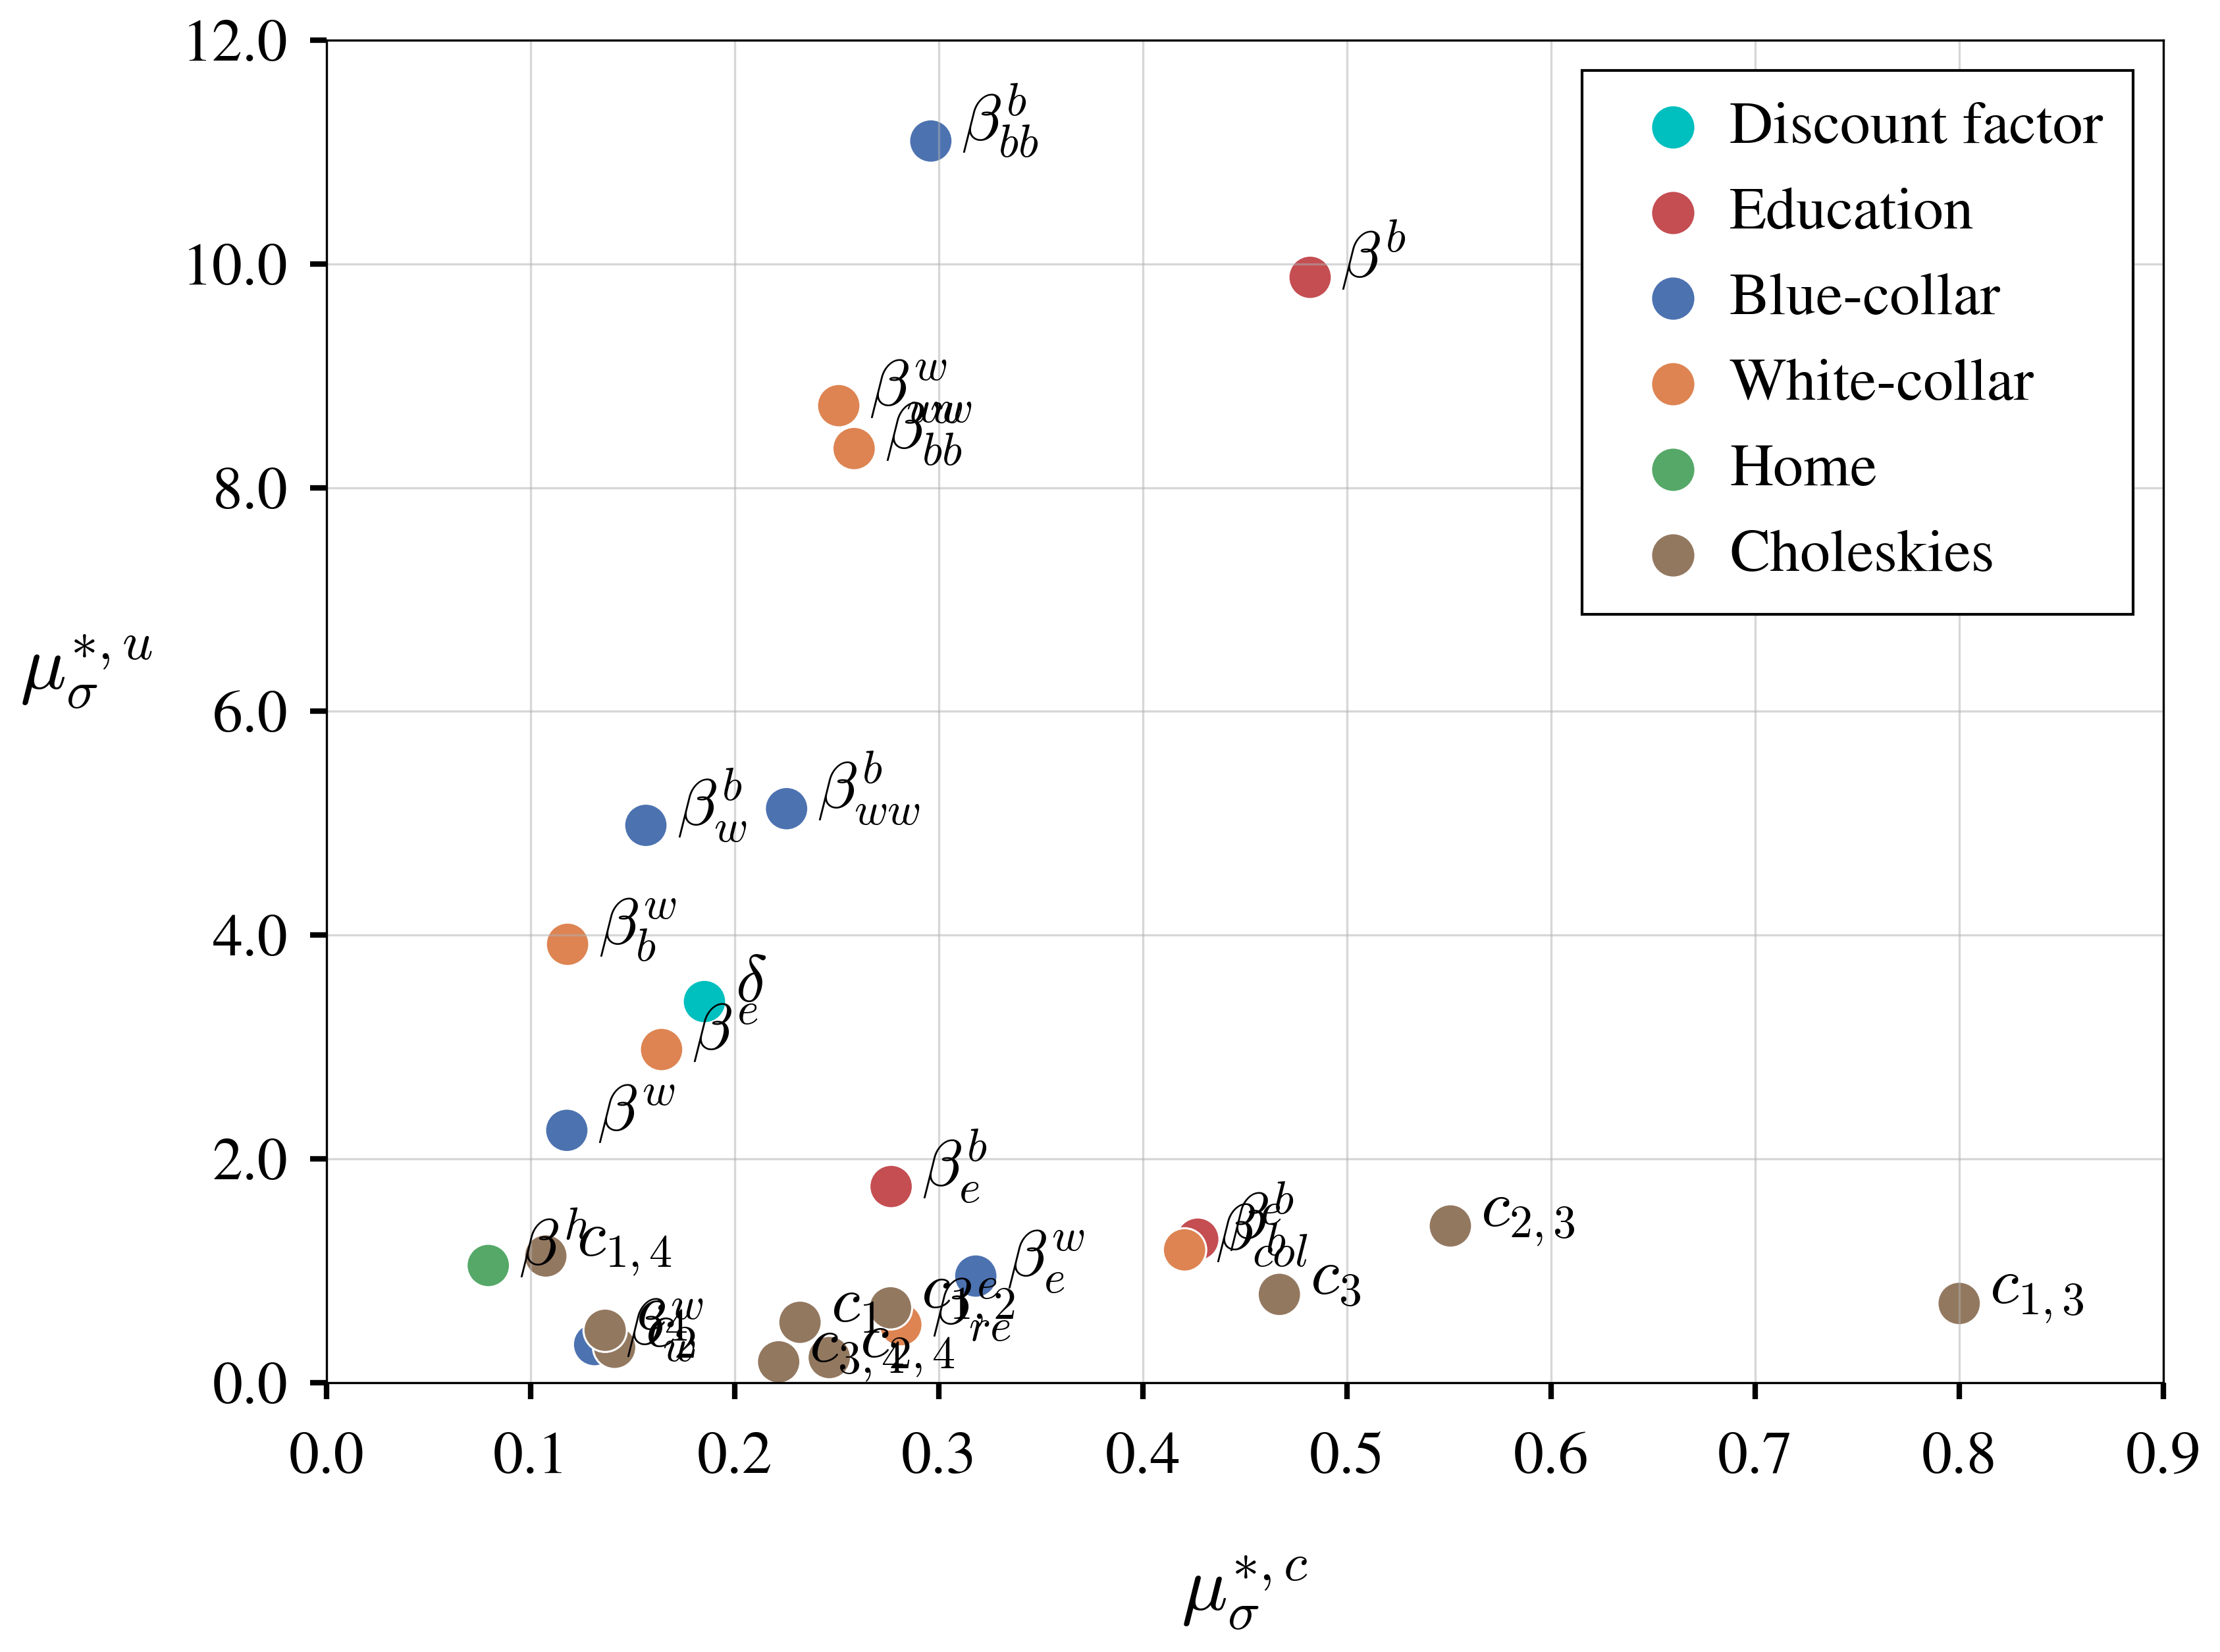
\includegraphics[scale=0.52]{../scrypy/figures/scatter_rad}
	\label{fig:rad}
\end{figure}


\begin{figure}[H]
	\caption[Sigma-normalized mean absolute EEs for trajectory design]{Sigma-normalized mean absolute Elementary Effects for trajectory design}
	\centering
	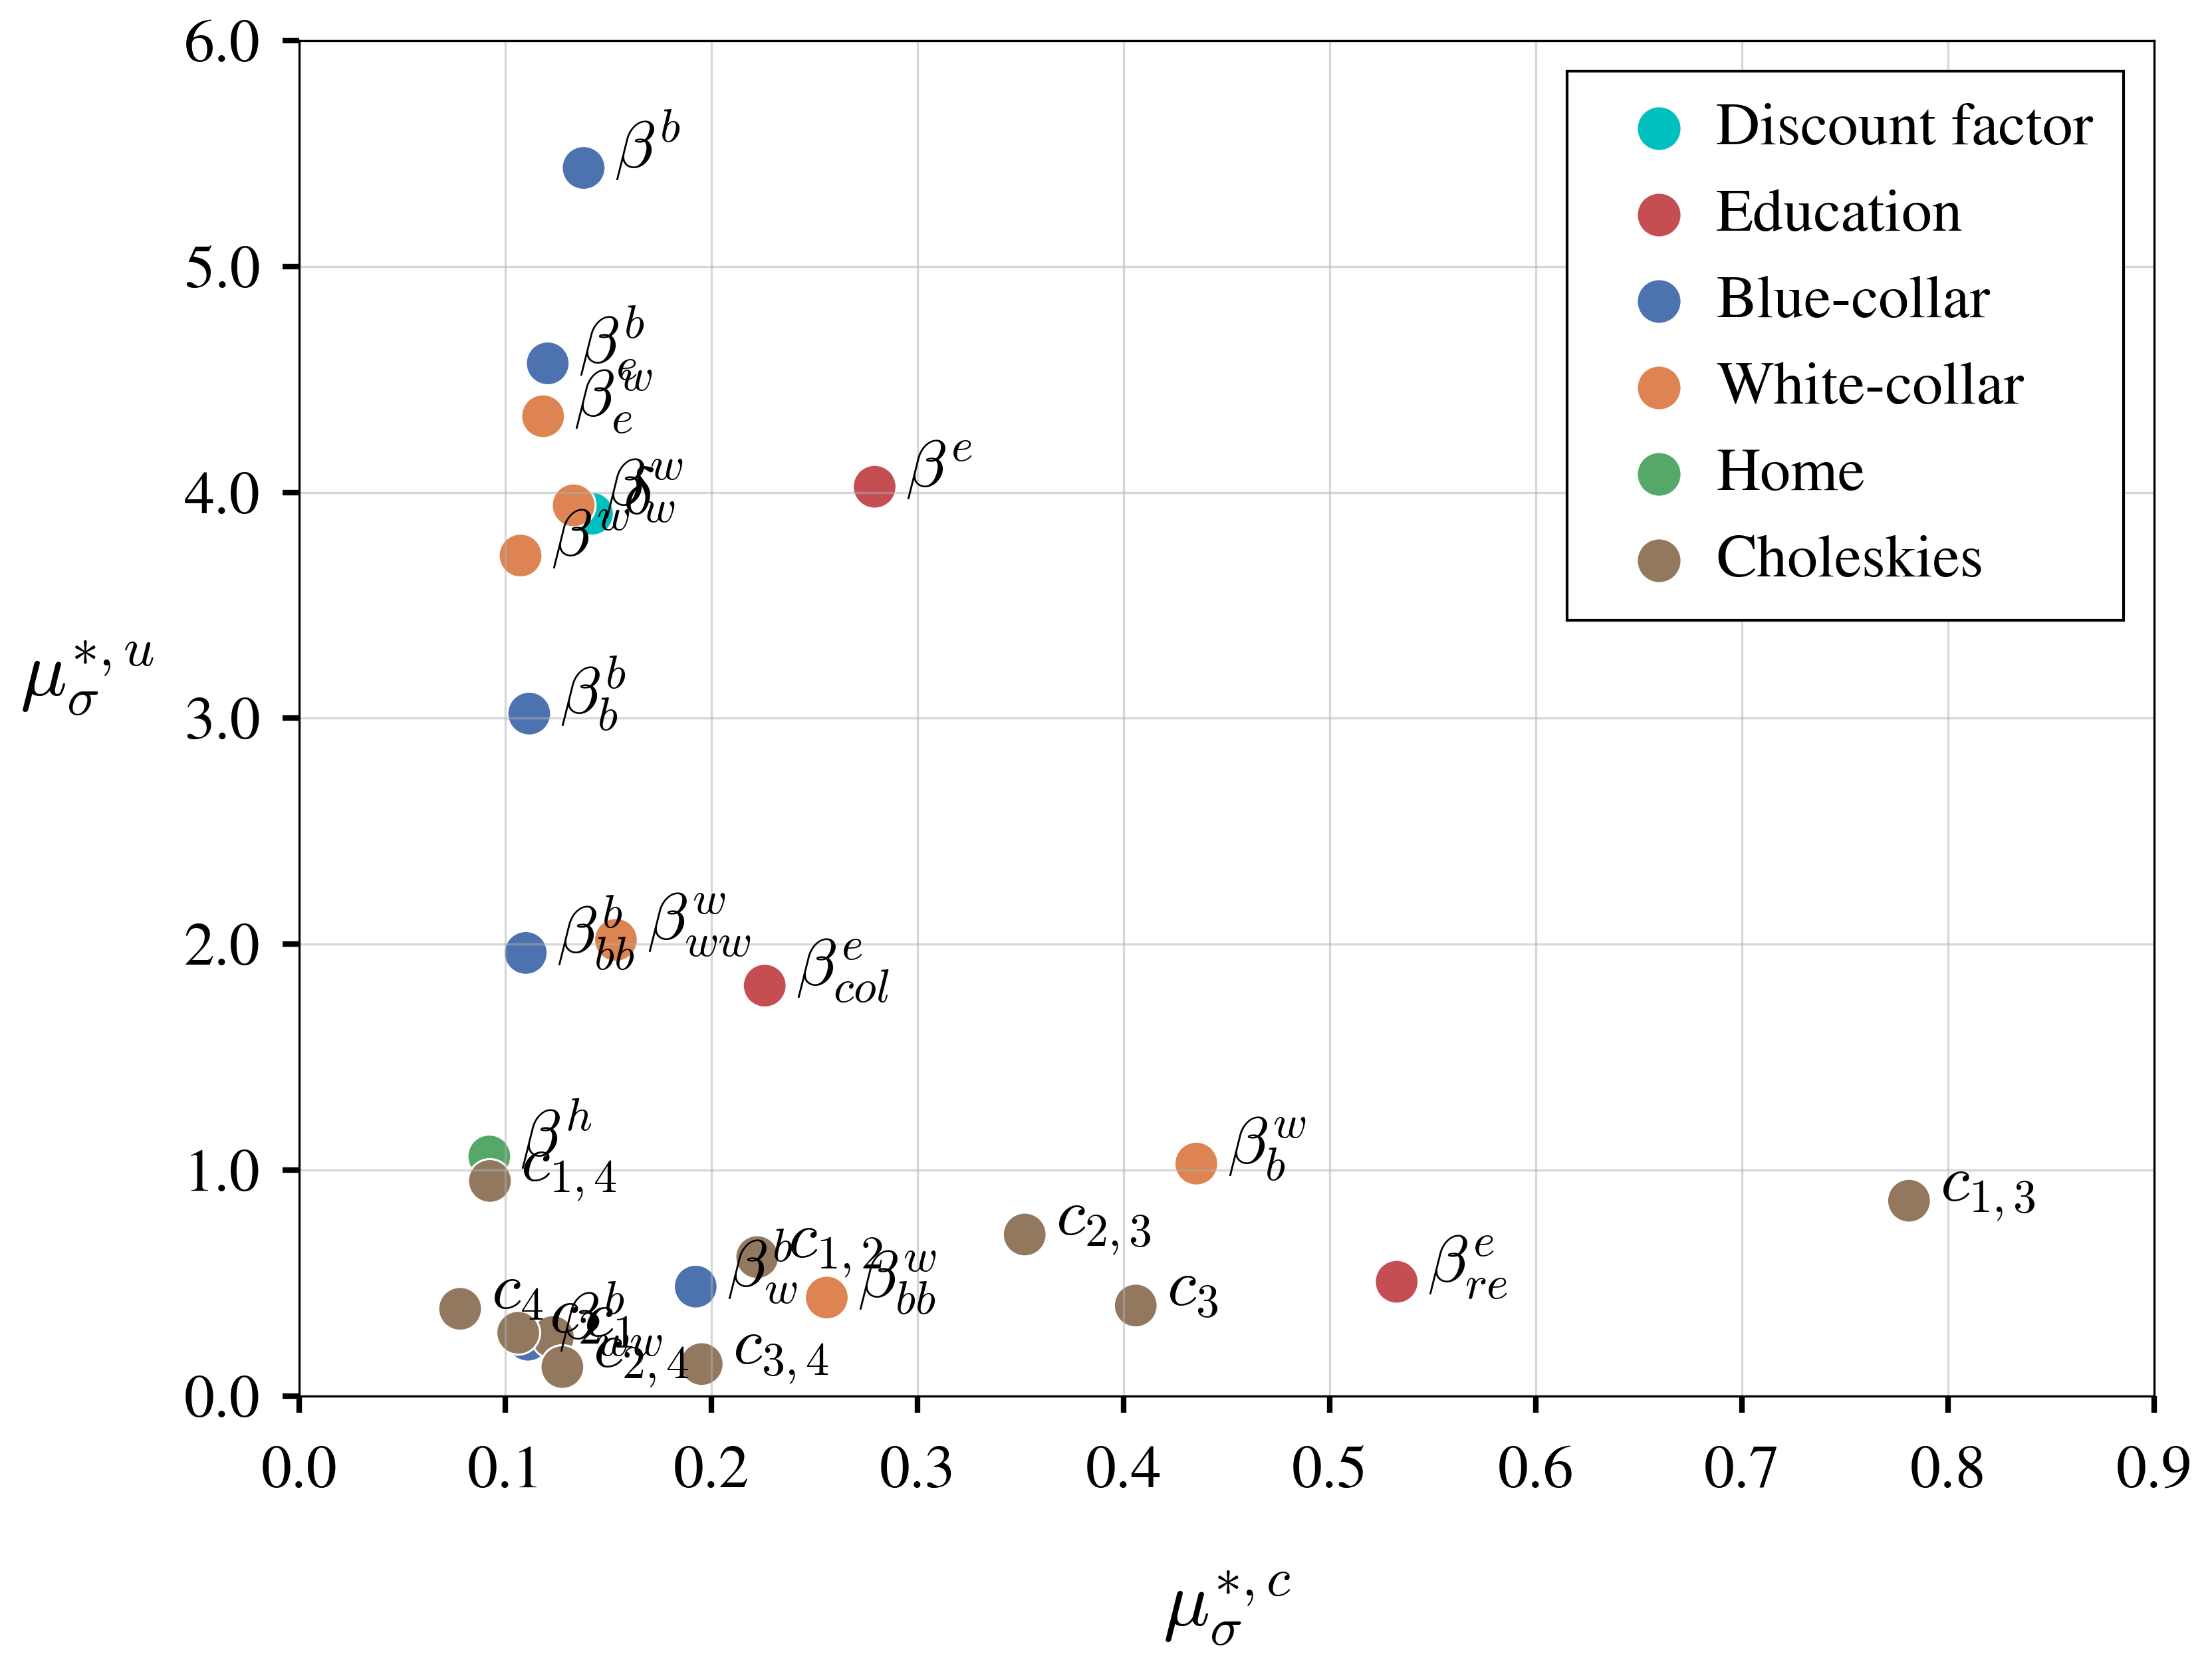
\includegraphics[scale=0.52]{../scrypy/figures/scatter_traj}
	\label{fig:traj}
\end{figure}
\newpage


\subsection{Appendix C: Simulated maximum likelihood estimation}
\thispagestyle{plain} % surpress header on first page
To estimate the exogenous model parameters, the approach that this thesis and also KW94 use is the simulated maximum likelihood method (\cite{Albright.1977})\footnote{See \cite{Aguirregabiria.2010}, p. 42-44 and \cite{Raabe.2019}, p. 21-26 for more details.}.

This method can be applied to a set of longitudinal data on occupational choices $a_t$ and, if available, wages $W_{a,t}^{-}$ of a sample of $i \in I$ individuals starting from age 16. To distinguish from its functional form, let $\mathcal{W}^{-}_{a(k),t}$ denote the measured wages. For each period $t$, the recorded choices $a_0$, ..., $a_{t-1}$  imply the occupation-specific experiences $x_{a,t}$. Together with $t$, they constitute the observable state vector $\bold{s_t^-}$. Consequently, the measured, observable endogenous variables are $\pmb{\mathcal{D}}\defeq(\bold{s_t^-},\mathcal{W}^{-}_{a,t})$. Given this setup, the goal is to estimate the exogenous model parameters $\pmb{\theta}\defeq(\delta, \pmb{\beta}, \pmb{\Sigma_\varepsilon})$.\footnote{Improvements in this thesis' estimation over KW94 are that, first, it is not assumed that the standard errors of the parameters estimates are uncorrelated, and, second, that $\beta$ is not left out of the estimation.} Thus, every probability is a function of the exogenous model parameters $\pmb{\theta}$.
The approach to compute the likelihood function $L_{\pmb{\mathcal{D}}}(\pmb{\theta})$ of the observables in the data begins with the individual latent variable representation in period $t$. The optimal choice is given by
\begin{align}
a_t = \argmax_a V(\bold{s_t^-},\pmb{\varepsilon_t},a_t),
\end{align}
As $a_t$ and $\bold{s_t^-}$ are known, the next step is to derive the unobservable shocks $\pmb{\varepsilon_t}$ in terms of $a_t$ and $\bold{s_t^-}$. Therefore, write the set of shocks for which the alternative-specific value function $V(\bold{s_t^-},\pmb{\varepsilon_t},a_t(j))$ is higher than the other value functions $V(\bold{s_t^-},\pmb{\varepsilon_t},a_t(k\neq j))$ as
\begin{align}
\pmb{\varepsilon_t}(a_t(j),\bold{s_t^-}) \defeq \{\pmb{\varepsilon_t}|V(\bold{s_t^-},\pmb{\varepsilon_t},a_t(j)) = \max_{a_t} V(\bold{s_t^-},\pmb{\varepsilon_t},a_t)\}).
\end{align}
Note that the set condition is a function of the unobservable model parameters $\pmb{\theta}$.

Consider first the case of non-working alternatives $a_t(j) \in [e,h]$. The probability of choosing $a_t(j)$ is the probability of set $\pmb{\varepsilon_t}(a_t(j),\bold{s_t^-})$. This probability equals the integral of the probability distribution function $f(\pmb{\varepsilon_t})$ over all elements of set $\pmb{\varepsilon_t}(a_t(j),\bold{s_t^-})$ with respect to $\pmb{\varepsilon_t}$. Formally,
\begin{align}
\text{p}\big(a_t(j) | \bold{s_t^-}\big) = \int_{\pmb{\varepsilon_t}(a_t(j),\bold{s_t^-})} f(\pmb{\varepsilon_t}) d^{|A|} \pmb{\varepsilon_t}.
\end{align}
\noindent
The second case is $a_t(k) \in [b,w]$. Assuming the dataset contains wages for the working alternatives $a_t(k)$, the probabilities of choosing $a_t(k)$ take a few steps more to compute. First, note from the wage equations that the alternative-specific shocks $\pmb{\varepsilon_{a,t}}$ are normally distributed. Second, in contrary to the non-working alternatives, using (\ref{eq:returns_b_w}), the shocks can directly be expressed as a function of the alternative-specific model parameters $\pmb{\beta_{a(k)}}$ by inserting the inferred alternative-specific experiences $\pmb{x_{a(k),t}}$ into $W_{a(k),t}$ and subtracting the expression from the observed wage $\mathcal{W}^{-}_{a(k),t}$ for each individual. Both wages are logarithmized. Thus,
\begin{align} \label{eq:epsilon}
\varepsilon_{a(k),t} = \text{ln}(\mathcal{W}^{-}_{a(k),t}) - \text{ln}(W_{a(k),t}^{-}).
\end{align}
Third, the alternative-specific shocks $\pmb{\varepsilon_{a,t}}$ are not distributed independently. Since $\varepsilon_{a(k),t}$ can be inferred from the
observed wage $\mathcal{W}^{-}_{a(k),t}$, this information can be used to form the expectation about the whole error distribution. Therefore, using the conditional probability density function $f(\pmb{\varepsilon_t}|\varepsilon_{a(k),t})$, the probability of choosing occupation $a_t(k)$ conditional on observed states and wages writes

\noindent
\begin{align} \label{eq:prob-choice}
\text{p}\big(a_t(k) | \bold{s_t^-},W^{-}_{a(k),t}\big) = \int_{\pmb{\varepsilon_t}(a_t(k),\bold{s_t^-})} f(\pmb{\varepsilon_t}|\varepsilon_{a(k),t}) d^{|A|} \pmb{\varepsilon_t}.
\end{align}
Applying integration by substitution yields the following expression for the probability of the observed wage:\footnote{See \cite{Raabe.2019}, p. 29, 39-40 for a complete derivation.}
\begin{align} \label{eq:prob-wage}
\text{p}\big(\mathcal{W}^{-}_{a(k),t} | \bold{s_t^-}\big) = \omega_t^{-1} \frac{1}{\sigma_{a(k)}} \phi\bigg(\frac{\varepsilon_{a(k),t}}{\sigma_{a(k)}}\bigg).
\end{align}
Here, $\omega_t^{-1}$ is the Jacobian of the transformation from observed wage $\mathcal{W}^{-}_{a(k),t}$ to error $\varepsilon_{a(k),t}$ in (\ref{eq:epsilon}) and $\phi$ is the standard normal probability density function.
Finally, the joint probability of observing choice $a_t(k)$ and wage $\mathcal{W}^{-}_{a(k),t}$ conditional on the observed states is given by the product of the two probabilities in (\ref{eq:prob-choice}) and (\ref{eq:prob-wage}):
\begin{align}
\text{p}\big(a_t(k),\mathcal{W}^{-}_{a(k),t}|\bold{s_t^-}\big) = \text{p}\big(a_t(k)|\bold{s_t^-}, \mathcal{W}^{-}_{a(k),t}\big)\text{p}\big(\mathcal{W}^{-}_{a(k),t}|\bold{s_t^-}\big).
\end{align}
Based on these results, the likelihood contribution $L^{i}_{\pmb{\mathcal{D}}}$ of one individual $i$ can be written as the product of the probability to observe the measured endogenous variables for one individual and for one period over all time periods:
\begin{align}
L^{i}_{\pmb{\mathcal{D}}}(\pmb{\theta}) = P\big(\{a_{t,}^{i},\mathcal{W}^{-,i}_{a,t,}\}_{t=0}^T\big) = \prod_{t=0}^{T} \text{p}\big(a_t^{i},\mathcal{W}_{a,t}^{-,i}|\bold{s_t^{-,i}}\big).
\end{align}
Therefore, the sample likelihood is given by the product of the individual likelihoods over the whole sample of individuals:
\begin{align} \label{eq:sample-likelihood}
L_{\pmb{\mathcal{D}}}(\pmb{\theta}) = P\big(\big\{\{a_{t,}^{i},\mathcal{W}^{-,i}_{a,t,}\}_{t=0}^T\big\}_{i \in I}\big) = \prod_{i \in I}\prod_{t=0}^{T} \text{p}(a_t^{i},\mathcal{W}_{a,t}^{-,i}|\bold{s_t^{-,i})}.
\end{align}
Since the probabilities are functions of the exogenous parameters $\pmb{\theta}$, the simulated maximum likelihood estimator $\pmb{\hat{\theta}}$ is the vector of exogenous parameters that maximizes (\ref{eq:sample-likelihood}). As the maximum likelihood estimator can be shown to be asymptotically normal under some regularity conditions\footnote{This property is an advantage of this thesis' estimation approach. It facilitates the uncertainty quantification via Monte Carlo sampling because there is a simple closed form for the (marginal) probability density available. This eases the construction of the desired samples.}, these results are taken as the mean vector for the input parameters in the uncertainty quantification.

The procedure to estimate the parameter vector $\pmb{\theta}$ using the expressions for the likelihood is as follows: first, The optimization algorithm of choice proposes a parameter vector. Second, the model is solved via backward induction. Third, using the policy functions, the likelihood is computed. These steps are repeated until the optimizer has found the parameter vector that yields the maximal likelihood.\\
\newline
Finally, the calculation of the estimator's covariance is described.\footnote{See \cite{Verbeek.2012}, p. 184-186.} The result is used as the covariance matrix for the input parameters in the UQ.

Under regularity conditions, the asymptotic covariance of a maximum likelihood estimator equals the inverse of the Fisher information matrix $\mathcal{I}(\theta)^{-1}$: $\text{Var}(\theta)=\mathcal{I}(\theta)^{-1}$. In this thesis, the information matrix $\mathcal{I}(\pmb{\theta})$ is given by the variance of the scores of the parameters.\footnote{The computation of $\text{Cov}(\pmb{\theta})$ by using the Jacobian of the individual likelihood contributions is chosen over other approaches because, first, it yields no error in the inversion step of $\mathcal{I}(\pmb{\theta})$ and, second, the results are reasonably close to the similar specification in KW94.} The scores $\text{s}(\pmb{\theta})$ are the first derivatives of the likelihood function. This can be written in terms of sample and individual likelihoods. Formally, the relationships are given by
\begin{align} \label{eq:scores}
\text{s}(\pmb{\theta}) \defeq \frac{\partial L_{\pmb{\mathcal{D}}}({\pmb{\theta}})} {\partial \pmb{\theta}} = \sum_{i \in I} \frac{L_{\pmb{\mathcal{D}}}^{i}(\pmb{\theta})}{\partial \pmb{\theta}} \defeq \sum_{i \in I}\text{s}_i(\pmb{\theta}).
\end{align}
Having multiple individual likelihood contributions, the scores are in the form of the  Jacobian matrix.
Using the property that the expected values of scores, $\E[\text{s}(\theta)]$, are zero at the maximum likelihood estimator. The variance of the scores is given by (\ref{eq:info-matrix}). It is equal to the inverse of the Fisher information matrix.
\begin{align} \label{eq:info-matrix}
\mathcal{I}^{-1}(\pmb{\theta}) = \text{Var}(\text{s}(\pmb{\theta})) = \E[\text{s}(\pmb{\theta})\text{s}(\pmb{\theta})'].
\end{align}
Hence, the estimator for the asymptotic covariance of the maximum likelihood estimator can be written as
\begin{align} \label{eq:est-cov}
\hat{\text{Cov}_J}(\pmb{\hat{\theta}}) = \bigg( \frac{1}{|I|} \sum_{i \in I} \text{s}_i(\pmb{\hat{\theta}})\text{s}_i(\pmb{\hat{\theta}})' \bigg)^{-1},
\end{align}
where $|I|$ is the number of individuals contained in the data set.
The intuition behind the above expression is the following: Estimator $\pmb{\hat{\theta}}$ maximizes the sample likelihood. This is equivalent to $\pmb{\hat{\theta}}$ setting the sample scores to zero. However, the individual likelihood may not be zero at the optimal parameter vector for the sample likelihood. This variation is captured by the variance of the individual scores evaluated at $\pmb{\hat{\theta}}$. The relations in (\ref{eq:scores}) and (\ref{eq:info-matrix}) then imply that the inverse of the variance of the individual scores is equivalent to the variance of the maximum likelihood estimator.